% Unified multimodal decoder — TikZ source. Compiles to a tight standalone PDF
% (pdflatex figures/unified-decoder.tex), which `book-scaffold build-figures`
% converts to public/figures/unified-decoder.svg.
%
% One decoder-only body over an interleaved text/image-code stream. Modality
% lives only at the modality-indexed embedding (bottom) and the routed head (top).
\documentclass[tikz,border=3pt]{standalone}
\usepackage{amsmath}
\usepackage{amssymb}
\usepackage{tikz}
\usetikzlibrary{positioning,arrows.meta,calc,fit}
\begin{document}
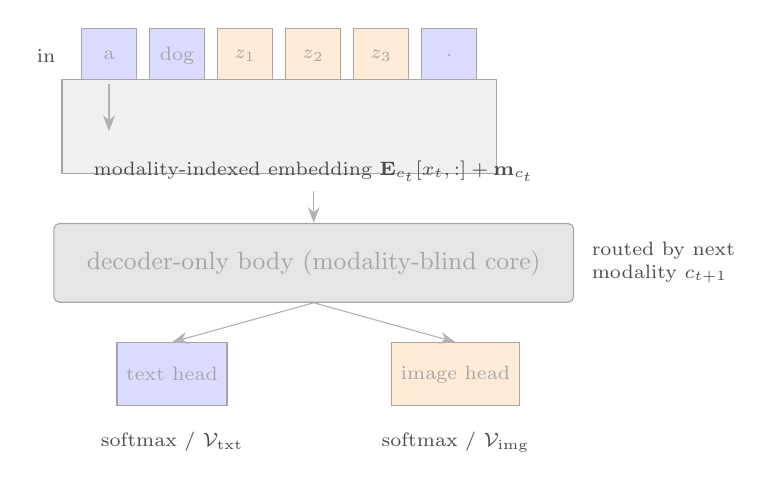
\begin{tikzpicture}[
    font=\small,
    tok/.style={draw, gray!70, minimum size=7mm, inner sep=1pt, font=\scriptsize},
    txt/.style={tok, fill=blue!14},
    img/.style={tok, fill=orange!16},
    op/.style={->, >={Stealth[length=2.0mm]}, gray!60},
  ]
  % input stream (interleaved)
  \node[txt] (i1) {a};
  \node[txt, right=1.5mm of i1] (i2) {dog};
  \node[img, right=1.5mm of i2] (i3) {$z_1$};
  \node[img, right=1.5mm of i3] (i4) {$z_2$};
  \node[img, right=1.5mm of i4] (i5) {$z_3$};
  \node[txt, right=1.5mm of i5] (i6) {.};
  \node[left=2mm of i1, font=\scriptsize, text=black!70] {in};

  % embedding row
  \node[draw, gray!70, fill=black!6, fit=(i1)(i6), inner sep=2.4mm,
        yshift=-9mm, minimum width=1mm] {};
  \node[below=8.5mm of i1, xshift=2.6cm, font=\scriptsize, text=black!70]
    (emb) {modality-indexed embedding $\mathbf E_{c_t}[x_t,:]+\mathbf m_{c_t}$};

  % body
  \node[draw, gray!70, rounded corners=2pt, fill=black!10,
        minimum width=6.6cm, minimum height=10mm, below=4mm of emb]
    (body) {decoder-only body (modality-blind core)};

  % routed heads
  \node[draw, gray!70, fill=blue!14, below=5mm of body, xshift=-1.8cm,
        minimum height=8mm, font=\scriptsize] (htxt) {text head};
  \node[draw, gray!70, fill=orange!16, below=5mm of body, xshift=1.8cm,
        minimum height=8mm, font=\scriptsize] (himg) {image head};
  \node[below=2mm of htxt, font=\scriptsize, text=black!70]
    {softmax / $\mathcal V_{\mathrm{txt}}$};
  \node[below=2mm of himg, font=\scriptsize, text=black!70]
    {softmax / $\mathcal V_{\mathrm{img}}$};

  \draw[op] (i1.south) -- ($(i1.south)+(0,-6mm)$);
  \draw[op] (emb) -- (body);
  \draw[op] (body.south) -- (htxt.north);
  \draw[op] (body.south) -- (himg.north);
  \node[right=1mm of body.east, font=\scriptsize, text=black!70, align=left]
    {routed by next\\modality $c_{t+1}$};
\end{tikzpicture}
\end{document}
